\begin{enumerate}
	\item 
		\begin{minipage}[t]{\linewidth}
		\raggedright
		\adjustbox{valign=t}{%
			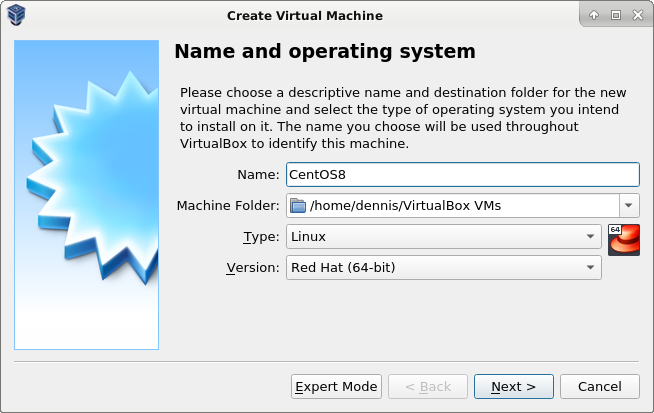
\includegraphics[width=0.99\linewidth]{linuxreader-img004.png}%
		}
		Noem de machine CentOS8 of een leuke eigen naam. Laat de Machine Folder naam zoals deze op jou machine is en ga hem niet aan passen naar wat er in de screenshot staat. Het Type systeem is Linux en de Version wordt Red Hat (64-bit).
		\end{minipage}
	\item Kies voor een 15 GB harddisk (VDI) die dynamisch mag groeien. Voor het geheugen gebruiken we 2 GB RAM.
	\item Als de machine aangemaakt is gaan we de netwerk settings wijzigen. We selecteren de machine en clicken op Properties. Bij Settings kiezen we voor Network.
	\item
		\begin{minipage}[t]{\linewidth}
		\raggedright
		\adjustbox{valign=t}{%
			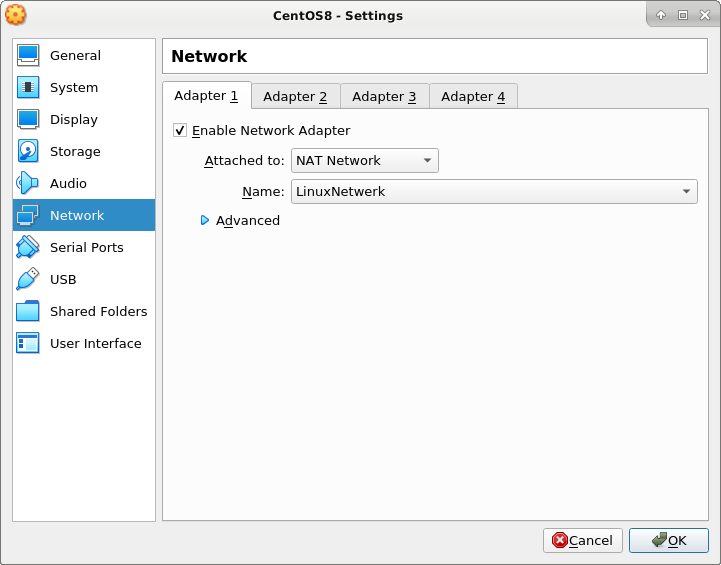
\includegraphics[width=0.99\linewidth]{linuxreader-img005.png}%
		}
		Wijzig bij Attached to: de setting naar NAT Network. Selecteer vervolgens bij Name: het LinuxNetwerk. Klik op OK om de gemaakte wijzigingen op te slaan.
		\end{minipage}
\end{enumerate}
